% !TEX root = ../main.tex

\chapter{Practical Implementation}
\label{ch:practical}

\emph{Part of this research has been described in a journal article in Digital Creativity in 2013, and I presented a paper at the Creativity and Cognition conference 2013 in Sydney.}

\grule % chktex 1

\todo{style inline code}
\todo{run code on laptop and get snippets of all variable contents, e.g.\ faustroll, froll\_dict, \ldots}
\todo{give examples of different results if using different base documents!}
\todo{add section about which pieces of code are not written by me}


The website \url{http://pata.physics.wtf} showcases the current proof-of-concept algorithms. This chapter gives an overview of the structure of the website and the development process.

Typically, software development is divided into so-called front and back ends. The frontend includes web design and web development and is meant to provide an interface for the end-user to communicate with the backend which involves a server, an application and a database (although this is not completely true in this project).

The frontend design is created using the \textbf{w3.css} stylesheet as a basis. The website is mostly responsive, meaning it can be viewed well on phones, tablets and screens (the poems and image spirals for example unfortunately have a fixed width which does not scale down well). The site contains various scripts written in \textbf{Javascript} (e.g. scramble letters, randomise poem, send email and tabbed content).\footnote{frontend links: \url{http://www.w3schools.com/w3css/}, \url{https://www.javascript.com/}}

The backend relies heavily on a \textbf{Python} framework called \textbf{Flask}. Most of the code is written in Python although some parts require a specific templating language called \textbf{Jinja} which renders content into HTML. The application uses several \acrshort{api}'s (Microsoft Translator, Bing, YouTube, Flickr, Getty and WordNet) and is version controlled using \textbf{Git}.\footnote{backend links: \url{https://www.python.org/}, \url{http://flask.pocoo.org/}, \url{http://jinja.pocoo.org/}, \url{https://git-scm.com/}}

The folder structure is as follows:

- app\\
--- static\\
----- css\\
----- images\\
----- corpus\\
--- templates\\
- .git\\
- dev.py\\
- guni.py\\
- live.py\\
- .gitignore\\
- README.md\\
- TODO.txt

\todo{folder structure}

\begin{comment}
  To provide a short overview, the tools’s workflow can be described as follows:
  \begin{enumerate}
    \item Tokenise texts and remove stopwords to build index,
    \item a query triggers the three pataphysical algorithms,
    \item each algorithm finds results for the query,
    \item retrieve some words before/after match for context, and
    \item render the resulting sentences.
  \end{enumerate}
\end{comment}

\todo{add audio? update this section depending on what i do}

From the homepage users can choose between text, image and video search. Then they can enter a query --- in the case of text search this should be single words only, image and video search support multi word queries.


\section{Corpus}

Instead of crawling the Internet the present tool uses a local collection of texts in its text-search. The corpus used resembles the fictional library of ``equivalent books'' from Alfred Jarry's \emph{Exploits and Opinions of Dr.\ Faustroll, $'$Pataphysician} \citeyear[p.10-12]{Jarry1996}\footnote{``In addition, three prints hanging on the walls, a poster by TOULOUSE-LAUTREC, \emph{Jane Avril}; one by BONNARD, advertising the \emph{Revue Blanche}; a portrait of Doctor Faustroll, by AUBREY BEARDSLEY\@; and an old picture, which appeared to us to be valueless, \emph{Saint Cado}, issued by the Oberthuer printing house of Rennes.''\parencite[p.12]{Jarry1996}}. In principle the \hypertarget{corpus}{corpus}\label{ref:corpus} is just a folder within the tool's directory structure which contains the following files:

\begin{enumerate}[start=0]
\item Alfred Jarry: \emph{Exploits and Opinions of Dr.\ Faustroll, $'$Pataphysician}
\item Edgar Allen Poe: \emph{Collected Works}
\item Cyrano de Bergerac: \emph{A Voyage to the Moon}
\item Saint Luke: \emph{The Gospel}
\item Leon Bloy: \emph{Le Desespere} (French)
\item Samuel Taylor Coleridge: \emph{The Rime of the Ancient Mariner}
\item Georges Darien: \emph{Le Voleur} (French)
\item Marceline Desbordes-Valmore: \emph{Le Livre des Meres et des Enfants} (French)
\item Max Elskamp: \emph{Enluminures} (French)
\item Jean-Pierre Claris de Florian: \emph{Les Deux Billets} (French)
\item \emph{One Thousand and One Nights}
\item Christian Grabbe: \emph{Scherz, Satire, Ironie und tiefere Bedeutung} (German)
\item Gustave Kahn: \emph{Le Conte de l'Or et Du Silence} (French)
\item Le Comte de Lautreamont: \emph{Les Chants de Maldoror} (French)
\item Maurice Maeterlinck: \emph{Aglavaine and Selysette}
\item Stephane Mallarme: \emph{Verse and Prose} (French)
\item Catulle Mendes: \emph{The Mirror} and \emph{la Divina Aventure} (English and Spanish)
\item Homer: \emph{The Odyssey}
\item Josephin Peladan: \emph{Babylon} (EMPTY FILE)\footnote{I have not been able to find any source texts online.\label{emptyfile}}
\item Francois Rabelais: \emph{Gargantua and Pantagruel}
\item Jean de Chilra: \emph{L'Heure Sexuelle} (EMPTY FILE)\textsuperscript{\ref{emptyfile}}
\item Henri de Regnier: \emph{La Canne de Jaspe} (EMPTY FILE)\textsuperscript{\ref{emptyfile}}
\item Arthur Rimbaud: \emph{Poesies Completes} (French)
\item Marcel Schwob: \emph{Der Kinderkreuzzug} (German)
\item Alfred Jarry: \emph{Ubu Roi} (French)
\item Paul Verlaine: \emph{Poems}
\item Emile Verhaeren: \emph{Poems}
\item Jules Verne: \emph{A Journey to the Centre of the Earth}
\end{enumerate}

The original list as it appears in ``Faustroll'' is shown below. Only three of the items have not been found as a resource. Some others have been approximated by using another text by the same author for example. Most of these were sourced from \textbf{Project Gutenberg}\footnote{\url{https://www.gutenberg.org/}} in their original languages.
\begin{enumerate}
\item BAUDELAIRE, a volume of E.A. POE translations.
\item BERGERAC, \emph{Works}, volume II, containing the \emph{Histrory of the States and Empires of the Sun}, and the \emph{History of Birds}.
\item \emph{The Gospel according to} SAINT LUKE, in Greek.
\item BLOY, \emph{The Ungrateful Beggar}.
\item COLERIDGE, \emph{The Rime of the ancient Mariner}.
\item DARIEN, \emph{The Thief}.
\item DESBORDES-VALMORE, \emph{The Oath of the Little Men}.
\item ELSKAMP, \emph{Illuminated Designs}.
\item An odd volume of the \emph{Plays} of FLORIAN\@.
\item An odd volume of \emph{The Thousand and One Nights}, in the GALLAND translation.
\item GRABBE, \emph{Scherz, Satire, Ironie und tiefere Bedeutung}, comedy in three acts.
\item KAHN, \emph{The Tale of Gold and of Silence}.
\item LAUTREAMONT, \emph{The Lays of Maldoror}.
\item MAETERLINCK, \emph{Aglavaine and Selysette}.
\item MALLARME, \emph{Verse and Prose}.
\item MENDES, \emph{Gog}.
\item \emph{The Odyssey}, Teubner's edition.
\item PELADAN, \emph{Babylon}.
\item RABELAIS\@.
\item JEAN DE CHILRA, \emph{The Sexual Hour}.
\item HENRI DE REGNIER, \emph{The Jasper Cane}.
\item RIMBAUD, \emph{The Illuminations}.
\item SCHWOB, \emph{The Childrens' Crusade}.
\item Ubu Roi.
\item VERLAINE, \emph{Wisdom}.
\item VERHAEREN, \emph{The Hallucinated Landscapes}.
\item VERNE, \emph{Voyage to the Center of the Earth}.
\end{enumerate}

\begin{fmpage}{\linewidth}
  \textbf{A note on copyright:}\\
  §5. Duration of copyright: ``For literary, dramatic, musical or artistic works 70 years from the end of the calendar year in which the last remaining author of the work dies.'' (\url{https://www.copyrightservice.co.uk/ukcs/docs/edupack.pdf})

  Maurice Maeterlinck and Marguerite Vallette-Eymery (a.k.a. Rachilde or Jean de Chilra) died less than 70 years ago and their work should still be under copyright. Alfred Jarry in the Simon Watson Taylor translation is a derivative work and is probably also still protected.  (\url{http://www.copyrightservice.co.uk/copyright/p22_derivative_works})

  §7. Mentions \emph{fair dealing}: ``Private and research study purposes'', so for the purposes of this project copyright should not apply.
\end{fmpage}

\begin{figure}[htbp]
  \centering
  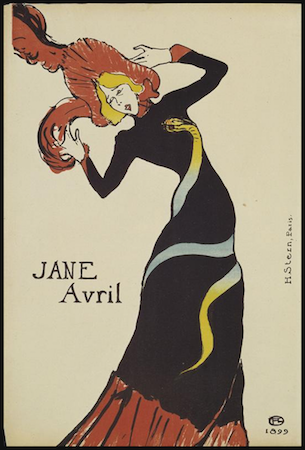
\includegraphics[width=\linewidth]{JaneAvril}
  \caption[Toulouse-Lautrec's ``Jane Avril'']{Toulouse-Lautrec's ``Jane Avril''}
\label{fig:toulouse}
\end{figure}

\begin{figure}[htbp]
  \centering
  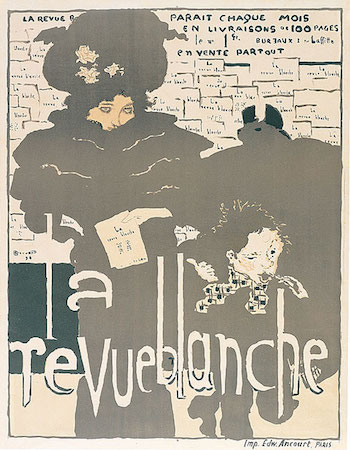
\includegraphics[width=\linewidth]{RevueBlanche}
  \caption[Bonnard's ``Revue Blanche'']{Bonnard's ``Revue Blanche''}
\label{fig:bonnard}
\end{figure}

\begin{figure}[htbp]
  \centering
  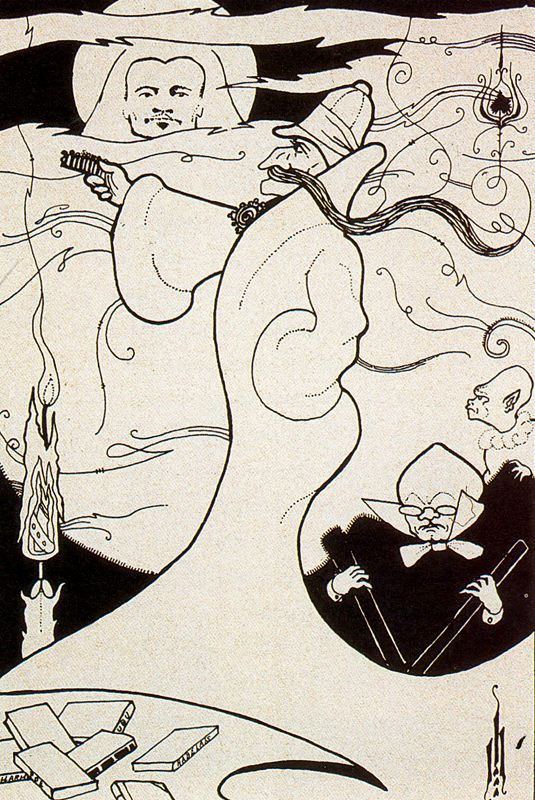
\includegraphics[width=\linewidth]{DocteurFaustroll}
  \caption[Aubrey Beardsley's ``Docteur Faustroll'']{Aubrey Beardsley's ``Docteur Faustroll''}
\label{fig:beardsley}
\end{figure}

\begin{figure}[htbp]
  \centering
  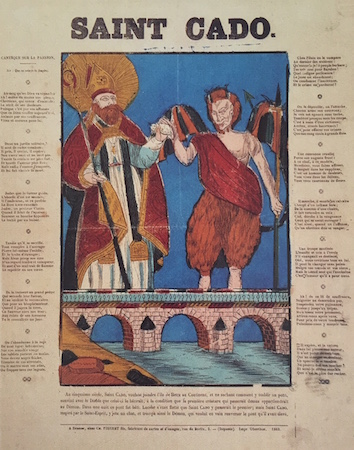
\includegraphics[width=\linewidth]{SaintCado}
  \caption[Oberthuer's ``Saint Cado'']{Oberthuer's ``Saint Cado''}
\label{fig:oberthuer}
\end{figure}


\section{Setup}

When the server is first started various setup functions are executed before any HTML is rendered. The search algorithms are triggered once a user enters a search term into the query field of any of the text, image or video pages.

Each plain text file in the corpus is processed. This means each word is added to a dictionary data structure together with the file ID's they occur in and a list of each position. Stopwords and non-alphabetic words are ignored (for a list of english stopwords see appendix~\ref{app:code}). After all files are read in the index looks like this:

\{\\
word1: \{fileA: [pos1, pos2, \ldots], fileB: [pos], \ldots\},\\
word2: \{fileC: [pos1, pos2], fileK: [pos], \ldots\},\\
\ldots\\
\}

Using one of the terms from figure~\ref{termdocs} on page~\pageref{termdocs}, here are their entries in the index file (the files are represented by their number in the \hyperlink{corpus}{corpus} (see page~\pageref{ref:corpus}), i.e. \textbf{l\_00} is the `Faustroll' file, \textbf{l\_01} is the `Poe' file, etc.). An excerpt from the actual file can be found in the appendix~\ref{app:code}.

\{\\
  doctor: \{\\
    l\_00: [253, 583, 604, 606, 644, 1318, 1471, 1858, 2334, 2431, 2446, 3039, 4743, 5034, 5107, 5437, 5824, 6195, 6228, 6955, 7305, 7822, 7892, 10049, 10629, 11055, 11457, 12059, 13978, 14570, 14850, 15063, 15099, 15259, 15959, 16193, 16561, 16610, 17866, 19184, 19501, 19631, 21806, 22570, 24867],\\
    l\_01: [96659, 294479, 294556, 294648, 296748, 316773, 317841, 317854, 317928, 317990, 318461, 332118, 338470, 340548, 341252, 383921, 384136, 452830, 453015, 454044, 454160, 454421, 454596, 454712, 454796, 454846, 455030, 455278, 455760, 455874, 456023, 456123, 456188, 456481, 456796, 457106, 457653, 457714, 457823, 457894, 458571, 458918, 458998, 459654, 459771, 490749],\\
    l\_02: [11476, 12098, 28151, 36270],\\
    l\_10: [53085, 53118, 53220, 53266, 53364, 53469, 53573, 53592, 53621, 53718, 54873, 55262, 55525, 55577, 55614, 55683, 55741, 56058, 62709, 113969, 114131, 114405, 114794],\
    l\_19: [14928, 15702, 49560, 82710, 167218, 180210, 189817, 189908, 190020, 190235, 190905, 199430, 226663, 275454, 275928, 278097, 287375, 291383, 304731, 306055, 324757, 330488],\\
    l\_27: [16270, 79245]\\
  \}, \ldots\\
\}


\section{Algorithms}

After the setup stage is completed and the webpage is fully loaded, user input in the form of a text query is required to trigger the three pataphysical algorithms.

Image and Video search do not use all three algorithms --- where relevant this is highlighted in each section. Generally the following descriptions refer to the text search functionality.


\subsection{Clinamen}

The clinamen is the unpredictable swerve that Bök calls ``the smallest possible aberration that can make the greatest possible difference'' \parencite{Boek2002}.

The clinamen algorithm works in two steps:
\begin{enumerate}
  \item get clinamen words based on dameraulevenshtein and faustroll
  \item get sentences from corpus that match clinamen words
\end{enumerate}

It uses the `faustroll' text by Alfred Jarry as a base document and the Damerau-Levenshtein algorithm \parencite{Damerau1964, Levenshtein1966}, which measures the distance between two strings (with 0 indicating equality), to find words that are similar but not quite the same. The distance is calculated using insertion, deletion, substitution of a single character, or transposition of two adjacent characters. This means that we are basically forcing the program to return matches that are of distance two or one, meaning they have two or one spelling errors in them.


\begin{equation}
  clinamen(t) = [v \colon 0 < dameraulevenshtein(t,v) \leq 2] \ \text{for} \ v \in V
\label{eq:clinamen}
\end{equation}
\myequations{clinamen}

Where:\\
\itab{$t$} \tab{is the query term,}\\
\itab{$V$} \tab{is the vocabulary of `faustroll',}\\




\subsection{Syzygy}

The syzygy surprises and confuses. It originally comes from astronomy and denotes the alignment of three celestial bodies in a straight line. In a pataphysical context it is the pun. It usually describes a conjunction of things, something unexpected and surprising. Unlike serendipity, a simple chance encounter, the syzygy has a more scientific purpose.

For the syzygy function, we made use of WordNet [29] through the NLTK python library [26] to find suitable results. Specifically, as shown in Eq. (2), the algorithm fetches the set of synonyms (synsets) first and then finds any hyponyms, hypernyms or holonyms for each of those (each of which denotes some sort of relationship or membership with its parent synonym). This mimics the syzygy alignment of three words in a line mentioned earlier (query $\to$ synonym $\to$ hypo/hyper/holonym).

This algorithm makes heavy use of WordNet. Line 1 creates a set of all synonyms for query term t from WordNet. It then loops through all individual items in the list of synonyms in line 2 to 5. Line 3 adds all hyponyms h for the current synonym s if there exists a word in the vocabulary same as the hyponym. Similarly lines 4 and 5 add all hypernyms and holonyms to the results list which is then returned in line 6.

\begin{lstlisting}
  Syzygy (t):
    synonyms = { s $\in$ WordNet-synsets (t) }
    for each s in synonyms:
      hypo   = { h: h $\in$ WordNet-hyponyms (s) }
      hyper = { h: h $\in$ WordNet-hypernyms (s) }
      holo    = { h: h $\in$ WordNet-holonyms (s) }
      union = hypo $\cup$ hyper $\cup$ holo
      add { h: h $\in$ union and $\exists$ h $\in$ V } to results
    return results
\end{lstlisting}

\begin{equation}
\begin{split}
  syzygy(t) &= \{ h \colon h \in union(t) \ \text{and} \ \exists \ h \in V \}\\% chktex 21
  union(t) &= hypo(t) \cup hyper(t) \cup holo(t)\\
  hypo(t) &= \{ h \colon h \in hyponyms(s) \}, \text{for} \ s \in syno(t)\\
  hyper(t) &= \{ h \colon h \in hypernyms(s) \}, \text{for} \ s \in syno(t)\\
  holo(t) &= \{ h \colon h \in holonyms(s) \}, \text{for} \ s \in syno(t)\\
  syno(t) &= \{ s \colon s \in synonyms(t) \}
\end{split}
\label{eq:syzygy}
\end{equation}
\myequations{syzygy}

\subsection{Antinomy}

The antimony, in a pataphysical sense, is the mutually incompatible.

For the antinomy we simply used WordNet’s antonyms (opposites) (see Eq. (3)). This function exhibits the same problem as mentioned above for the syzygy, just much worse.  Arguably, some words just do not appear to have an opposite, but the pataphysical antinomy should still be able to find a match. A better thesaurus or a larger index (e.g.\ based on more than one book – or, of course, the Web) could improve this method.

This algorithm is very similar to the algorithm for the syzygy. It finds all antonyms through WordNet and returns them if they appear in our dictionary of words.

\begin{lstlisting}
  Antinomy (t):
    synonyms = { s $\in$ WordNet-synsets (t) }
    for each s in synonyms:
      add { h $\in$ WordNet-antonyms (s): $\exists$ h $\in$ V } to results
    return results
\end{lstlisting}

\begin{equation}
  \begin{split}
  antinomy( t ) &= \{ h \colon h \in anto( t ) \ \text{and} \ \exists \ h \in V \}\\% chktex 21
  anto( t ) &= \{ h \colon h \in antonyms( s ) \}, \text{for} \ s \in syno( t )\\
  syno( t ) &= \{ s \colon s \in synonyms( t ) \}
  \end{split}
\label{eq:antinomy}
\end{equation}
\myequations{antinomy}







\section{Implementation}

Linking back to some of the creative, pataphysical concepts we have discussed earlier, let us put some of the ideas for our tool into perspective. The constraints for our conceptual space are the pataphysical rules that we want to apply to our data. We use those rules to explore, combine and transform our space; giving us the flexibility and freedom we need to find interesting results.

We developed the idea of pataphysicalising data as the process of applying such pataphysical rules in order to produce creative search results. This pataphysicalisation process forms a central component of our system (see Figure~\ref{fig:patasearch01}) and influences all areas of the search tool.

\todo{redraw figure}

\begin{figure}[htb] % (here, top, bottom, page)
  \centering
  \includegraphics[width=\linewidth]{images/patasearch01}
\caption[Pata central]{Pata central}
\label{fig:patasearch01}
\end{figure}

\begin{figure}[htb] % (here, top, bottom, page)
  \centering
  % \def\svgwidth{\columnwidth}
  \input{images/patasearch01.pdf_tex}
\caption[Pata central]{Pata central}
\label{fig:patasearch02}
\end{figure}


\section{User experience}

Whilst developing a system that returns creative results to the end user has numerous advantages, the assumptions that are made about and the decisions we take for the user must still be considered. For example, presume that the user inputs a search request `The Cat in the Hat' after reading a Dr.\ Seuss book to their child, and the system employs an anomalous method on the query and searched `sunglasses'. Whilst there is logic to the new search request, it is anomalous to the initial request, if the user receives these results without being told what method was used, the results will appear random, and therefore are likely to be detrimental to the user. Therefore the level of interaction the user has with the system and the feedback the system gives to the user on decisions it is making will have a large influence on the overall effectiveness and appreciation of the search tool. A quick and simple solution to this problem would be to add an icon to the side of each search result which displays how the original query was pataphysicalised.

\begin{figure}[htb] % (here, top, bottom, page)
  \centering
  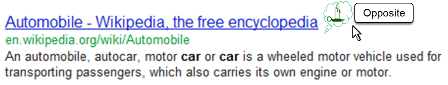
\includegraphics[width=\linewidth]{images/resultexample}
\caption[Feedback button]{Feedback button}
\label{fig:feedback}
\end{figure}

The above image (figure~\ref{fig:feedback}) shows an example of how this could be implemented. The little green candle (a reference to pataphysics in itself by the way) shows a pop-up note when hovered over with the mouse pointer. In this case the original query could have been `tree' and `car' was returned as an opposite to that.

\textbf{Results design}

Text
- Poetry
-- Queneau
-- Random
- Sources
- Algorithms

Images and Videos
- Spiral
- List




\section{Website}

\url{http://pata.fania.eu}

\url{http://pata.physics.wtf}


\section{APIs}

\begin{itemize}
  \item Bing
  \item YouTube
  \item Microsoft Translate
  \item Flickr
  \item WordNet
\end{itemize}


\section{Design}

\begin{itemize}
  \item random sentences
  \item spiral
  \item Word Scrable
  \item $\dots$
\end{itemize}


\section{Prototype 2}

{\Huge \url{pata.fania.eu}}

\begin{figure}[htb] % (here, top, bottom, page)
  \centering
  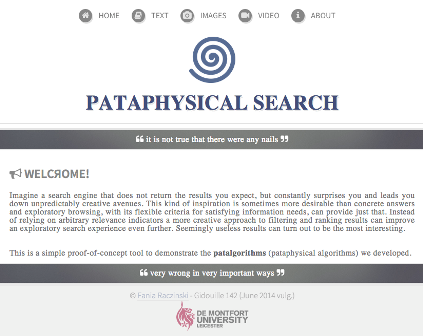
\includegraphics[width=\linewidth]{images/prototype02}
\caption[Prototype2]{Prototype2}
\label{fig:Prototype2x}
\end{figure}

\begin{alltt}
# TEXT

## setup

1.\ read in faustroll book
2.\ create `froll_dict' dictionary from text
3.\ remove stopwords and numbers from `froll_dict'

## text algorithm

1.\ get query term
2.\ execute three functions:

  2a.\ syzygy algorithm
    1.\ get list of synonyms
    2.\ for each synonym do the following:
      a.\ find hyponyms; if a hyponym occurs in `froll_dict' then add to the output list
      b.\ find hypernyms; if a hypernym occurs in `froll_dict' then add to the output list
      c.\ find holonyms; if a holonym occurs in `froll_dict' then add to the output list
    3.\ return list of syzygy words

  2b.\ antinomy algorithm
    1.\ get list of synonyms
    2.\ for each synonym do the following:
      a.\ find antonyms; if a antonym occurs in `froll_dict' then add to the output list
    3.\ return list of antinomy words

  2c.\ clinamen algorithm
    1.\ find list of words within `froll_dict' that have a `dameraulevenshtein distance' of 1 or 2 (meaning, there are 1 or 2 spelling errors)
    2.\ return list of clinamen words

3.\ get sentences for all three output lists

  3a.\ if the word appears in faustroll then find the nearest 5 words before and after the word
  3b.\ return list of sentences

4.\ render results as html


---

# IMAGES

## setup

- microsoft translate API key
- flickr API key
- (bing image search API key) --- not used atm

## image algorithm

1.\ get query word
2.\ get one syzygy word using syzygy algorithm 2a above
3.\ translation party
  3a.\ translate english to french
  3b.\ translate french to japanese
  3c.\ translate japanese to english
4.\ get images
  4a.\ search flickr for 10 matches to english translation
  4b.\ get metadata for each
  4c.\ add title, thumb, link to output list
5.\ return output list
6.\ render results as html

---

# VIDEOS

## setup

- microsoft translate API key
- youtube API stuff
- (bing video search API key) --- not used atm

## video algorithm

1.\ get query word
2.\ get one syzygy word using syzygy algorithm
3.\ translation party
  3a.\ translate english to french
  3b.\ translate french to japanese
  3c.\ translate japanese to english
4.\ get videos
  4a.\ search YouTube for 10 matches to english translation
  4b.\ get metadata for each
  4c.\ add title, thumb, link to output list
5.\ return output list
6.\ render as html
\end{alltt}


\section{Prototype 1}

\begin{figure}[htb] % (here, top, bottom, page)
  \centering
  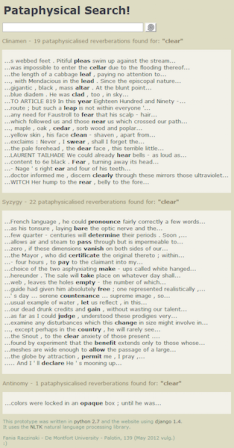
\includegraphics[height=0.6\textheight]{images/prototype01}
\caption[Prototype1]{Prototype1}
\label{fig:Prototype1x}
\end{figure}
